\documentclass[pdf,bluish,slideColor,colorBG]{prosper}
\hypersetup{pdfpagemode=FullScreen}
\usepackage{color}
\usepackage{graphicx}
\usepackage{amsfonts}
\usepackage{amsmath}
\def\baselinestretch{0.7}
\parindent 0.3in
\hyphenpenalty=10000
\tolerance=10000
\pagestyle{empty}

\def\Prob{{\rm Prob\;}}
\def\prob{{\rm \;Prob\;}}
\def\Var{{\rm Var}}        % Var
\def\Cov{{\rm Cov}}        % Cov

\DeclareSymbolFont{AMSb}{U}{msb}{m}{n}
\DeclareMathSymbol{\expect}{\mathalpha}{AMSb}{'105}

% bold math (use \bm{...})
\def\bm#1{\mathpalette\bmstyle{#1}}
\def\bmstyle#1#2{\mbox{\boldmath$#1#2$}}

\title{Differences between populations}

\author{Joe Felsenstein}

\institution{Biology 550D}

\subtitle{\small \\  7 December 2016}


\definecolor{orange}{rgb}{1.0,0.8,0.0}
\definecolor{Dandelion}{rgb}{0.8,0.4,0.3}
\definecolor{golden}{rgb}{1.0,0.75,0.2}
%\definecolor{golden}{rgb}{1.0,0.8,0.3}
\definecolor{purple}{rgb}{0.6,0.2,0.6}
\definecolor{darkblue}{rgb}{0.1,0.1,0.6}
\definecolor{yellow}{rgb}{1.0,1.0,0.0}
\definecolor{brightred}{rgb}{1.0,0.,0.0}
\definecolor{black}{rgb}{0.0,0.0,0.0}
\definecolor{white}{rgb}{1.0,1.0,1.0}
\definecolor{purple}{rgb}{0.8,0.0,0.8}

% sets backgroundcolor for whole document 
%\pagecolor{darkblue}
%\pagecolor{white}
% sets text color
%\color{yellow}
%\color{black}
% to change just a few words
% using \textcolor{color}{text}

\DeclareSymbolFont{AMSb}{U}{msb}{m}{n}
\DeclareMathSymbol{\expect}{\mathalpha}{AMSb}{'105}

\def\Prob{{\rm Prob\;}}
\def\prob{{\rm \;Prob\;}}
\def\Var{{\rm Var}}        % Var
\def\Cov{{\rm Cov}}        % Cov

\begin{document}


\maketitle

{
\parindent=0in

\overlays{4}{
\begin{slide}[Replace]{Evolutionary forces acting on populations}
\bigskip

\begin{itemstep}
\item Natural selection toward optima (which can differ between populations)
\item Genetic drift, making populations differ
\item Migration, making adjacent populations more similar
\end{itemstep}

\end{slide}
}

\begin{slide}[Replace]{An simulated example with no migration}
\bigskip

\centerline{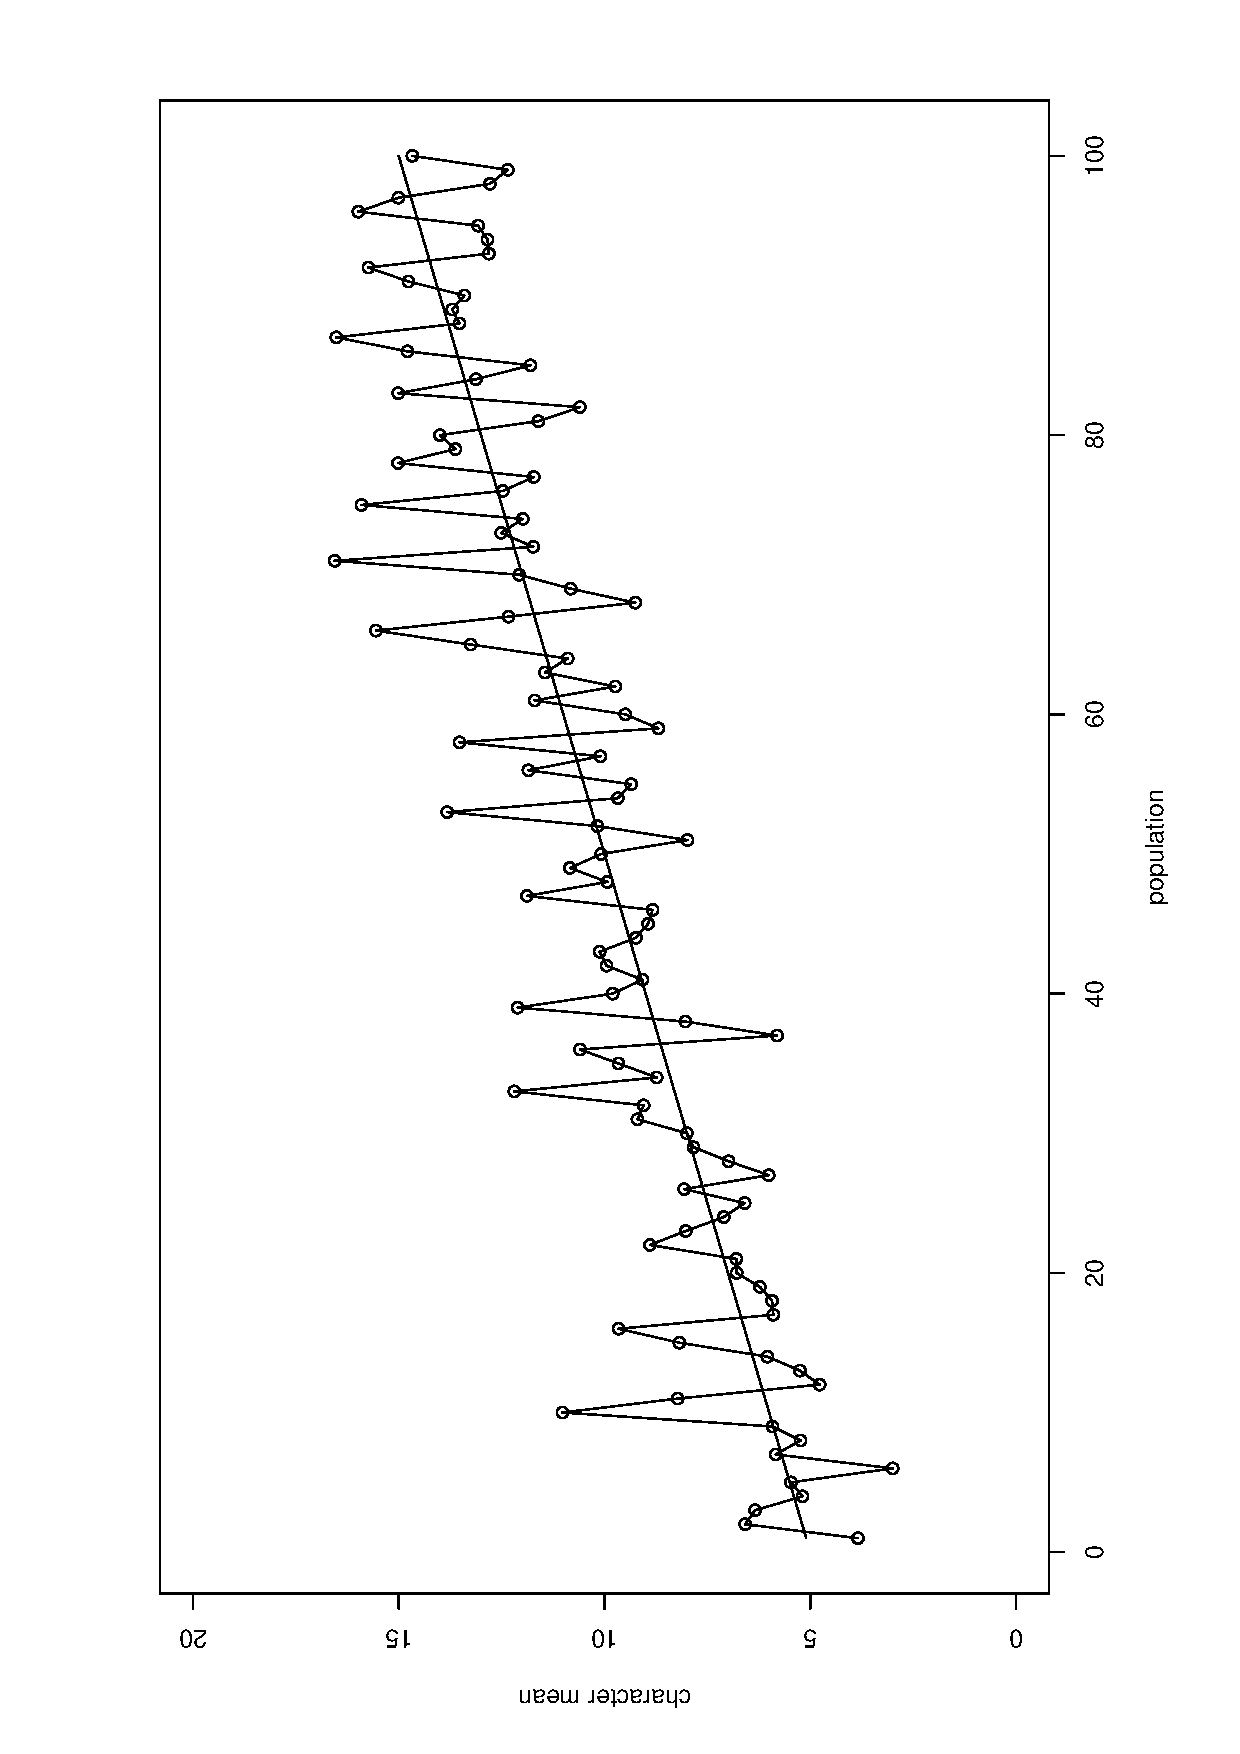
\includegraphics[height=2in]{driftselandm0.idraw}}

\end{slide}

\begin{slide}[Replace]{An simulated example with migration}
\bigskip

\centerline{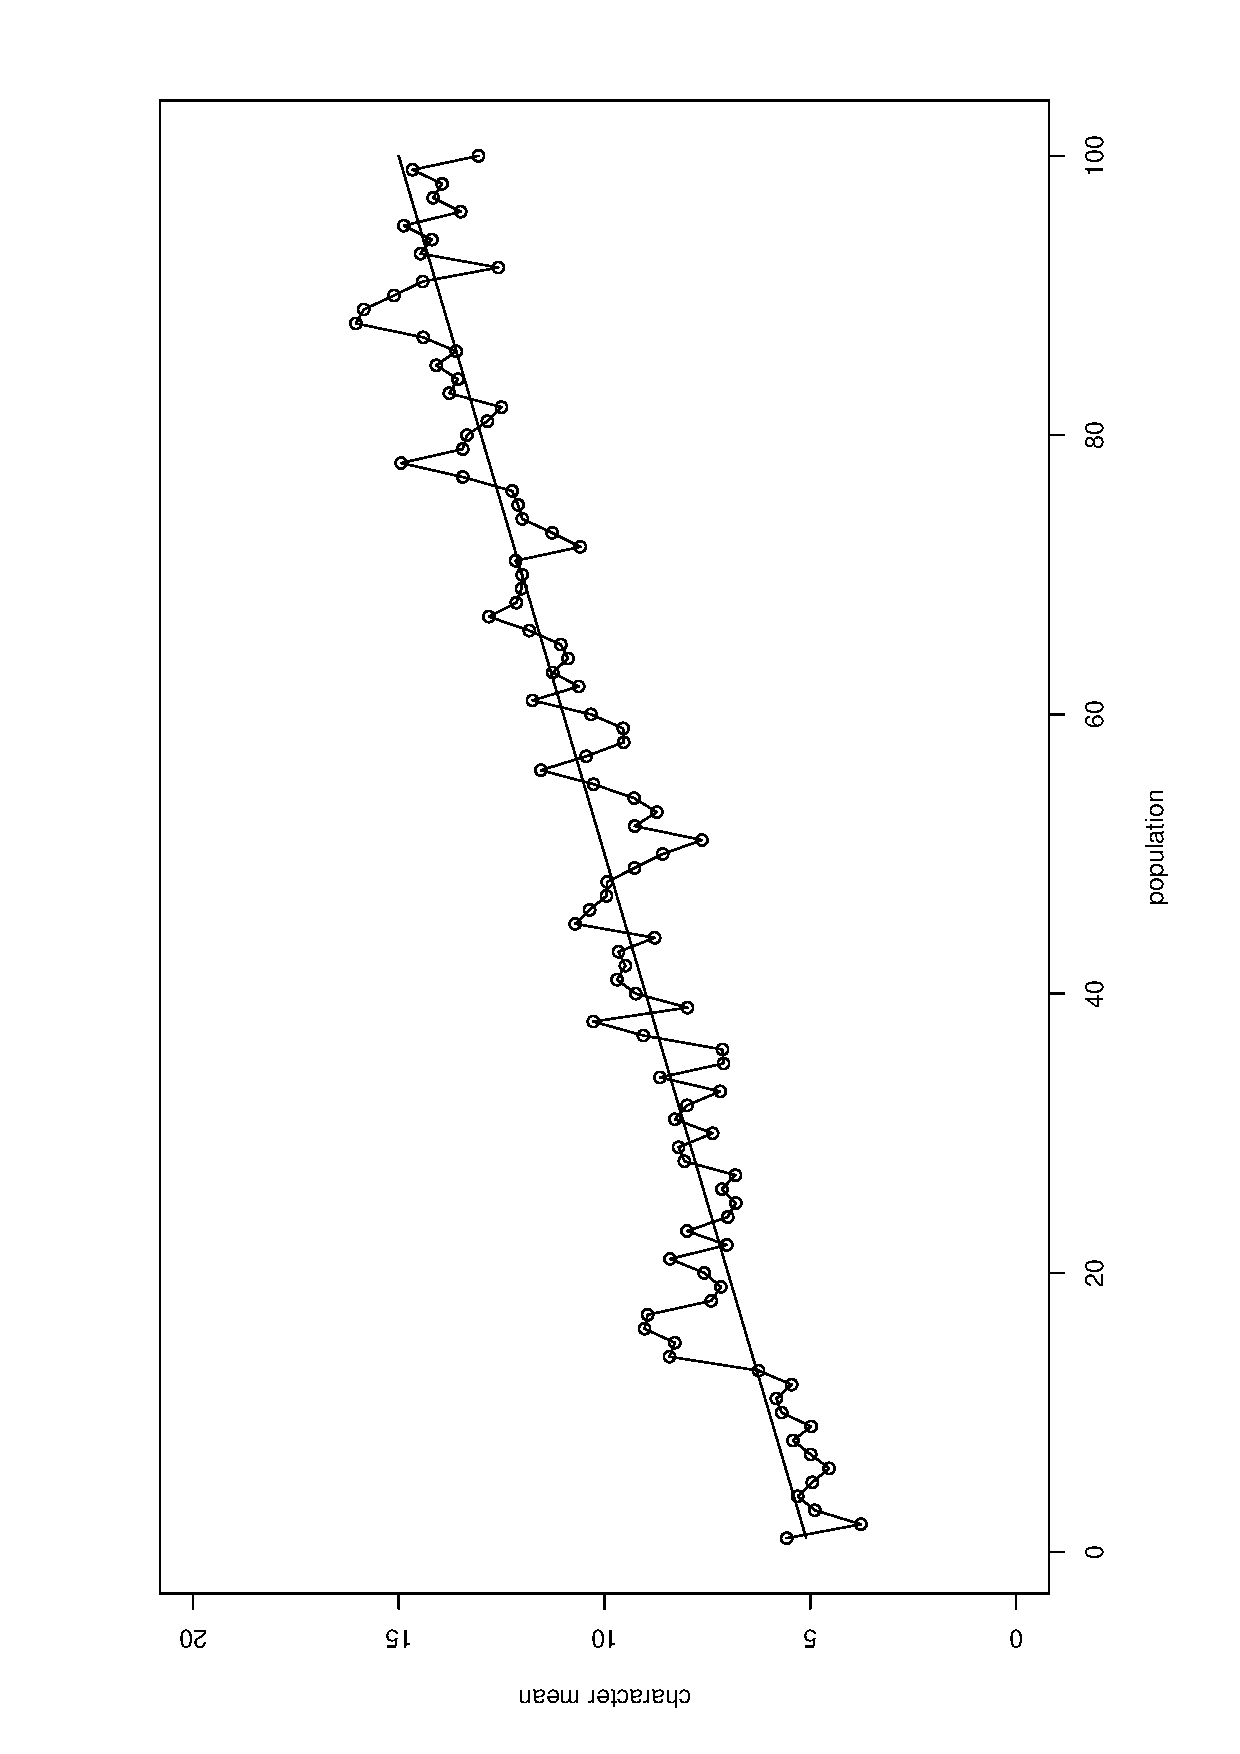
\includegraphics[height=2in]{driftselandm1.idraw}}

\end{slide}

\begin{slide}[Replace]{A geographic region with local migration}

\centerline{\includegraphics[width=2.2in]{migrex1.idraw}}

\end{slide}

\begin{slide}[Replace]{Phenotypes resulting from genetic drift alone}

\centerline{\includegraphics[width=2.2in]{migrex2.idraw}}

\end{slide}

\begin{slide}[Replace]{A more general migration matrix}
 
\centerline{\includegraphics[width=4in]{generalmatrix.idraw}}
 
\end{slide}
 
\begin{slide}[Replace]{13 populations and an environmental variable}

\centerline{\includegraphics[width=3in]{pop13.idraw}}
\bigskip

Simulated with $N = 100,\ \ m = 0.2,\ \ a = 10, \ \ b = 0.1, \ \ \sigma = 0.0001$

\end{slide}

\begin{slide}[Replace]{phenotype plotted against the environmental variable}
\bigskip

\centerline{\includegraphics[width=3.5in]{phenplot.idraw}}

\end{slide}

\begin{slide}[Replace]{contrasts of phenotype versus constrast of environment}
\bigskip

\centerline{\includegraphics[width=3.5in]{zplot.idraw}}

\end{slide}

\begin{slide}[Replace]{A numerical example with a 5-population matrix}

\centerline{\includegraphics[width=2.3in]{migr5.ydraw}}

\end{slide}

\begin{slide}[Replace]{The contrasts from that 5-population matrix}
\vspace{-0.5in}

\centerline{\includegraphics[width=2.8in]{migmatcont.ydraw}}

\end{slide}

\begin{slide}[Replace]{A simulated example}
\vspace{-0.8in}

\centerline{\includegraphics[width=2.8in]{cline.idraw}}
\bigskip

\centerline{(No selection, with $\mathsf{m = 0.01}$ and $\mathsf{\beta = 0.02}$)}

\end{slide}

\begin{slide}[Replace]{Its contrasts}

\centerline{\includegraphics[width=3in]{clinecontrasts.idraw}}

\end{slide}

\begin{slide}[Replace]{Fourier transform of characters}


When we have a linear ``stepping-stone" model of population
structure, the appropriate transform is simply the discrete Fourier
transform.  Migration damps the sine waves of different wavelengths
differently.  Here is a linear continuum with the optimum phenotype
curve the sum of three sine waves, and the corresponding curve of the
phenotypic means that results when migration damps them:
\vspace{-0.3in}

\centerline{\includegraphics[width=1.9in]{sinewaves2.idraw}}

\end{slide}

\begin{slide}[Replace]{A worry: direct effects of the environment}
\bigskip

If the responses to the environment are not genetic but are the direct effect
on the phenotype, we might get wrong inferences about selection.

\begin{itemize}
\item We could escape this by ``common garden'' experiments but this is hard.
\item There are statistical ways of detecting this -- basically that migration
among neighbors will not make them more similar than corresponding pairs of
populations that have the same two environments but are farther away from
each other. Power of inference?
\end{itemize}

\end{slide}

\begin{slide}[Replace]{Previous work}

Previous papers on this:
\begin{itemize}
\item Mal\'ecot (1949) and Kimura and Weiss (1964) used Fourier transforms
to solve for identity by descent in one- and two-dimensional infinite
stepping stone models of gene frequencies.
\item Much subsequent work by Takeo Maruyama (1971ff.) on this for finite
one- and two-dimensional stepping stone models.
\item Hansen, Armbruster and Antonsen ({\bf \it American Naturalist}, 2000) used Fourier transforms to correct
for migration in analyzing phenotypic data in one-dimensional stepping stone
models.  This work is in effect
a generalization of theirs to the general migration matrix model of Bodmer
and Cavalli-Sforza (1965).
\end{itemize}

\end{slide}

\begin{slide}[Replace]{Previous work, continued}

\begin{itemize}
\item Much of the present algebra was already published by me:
\begin{quote}
Felsenstein, J.  2002.  Contrasts for a
within-species comparative method.
pp.  118-129 in M. Slatkin and M. Veuille, 
{\bf \it Modern Developments
in Theoretical Population Genetics.}  Oxford University Press, Oxford.
\end{quote}
\item See also relevant agonizing about what we can infer about migration
matrices in my paper in Journal of Theoretical Biology, 1981.
\item Inference of migration matrices by sampling (IS and MCMC) methods:
papers by Beerli and Felsenstein (1999, 2001) and Bahlo and Griffiths (2000).
\end{itemize}

\end{slide}

\begin{slide}[Replace]{Furthermore ... }

Is there some way of thinking about how we can infer, from distributions of
gene frequencies, the whole set of migration matrices and historical
branching events that are not rejected?  This raises some very interesting
algebraic issues.
\bigskip

It is an example (like pedigree estimation and invariants of phylogenies)
of a highly structured set of hypotheses, all with the same number of
degrees of freedom, where we need to know which ones the data supports.
\bigskip

In this sense the problem is not so statistically simpleminded.

\end{slide}
}

\end{document}

